%%%%%%%%%%%%%%%%%%%%%%%%%%%%%%%%%%%%%%%%%%%%%%%%%%%%%%%%%%%%%%%%%%%%%%%%%%%%%%%%
\documentclass[twocolumn]{revtex4}

%%%%%%%%%%%%%%%%%%%%%%%%%%%%%%%%%%%%%%%%%%%%%%%%%%%%%%%%%%%%%%%%%%%%%%%%%%%%%%%%

\usepackage[]{graphicx}
%%%%%%%%%%%%%%%%%%%%%%%%%%%%%%%%%%%%%%%%%%%%%%%%%%%%%%%%%%%%%%%%%%%%%%%%%%%%%%%%

%%%%%%%%%%%%%%%%%%%%%%%%%%%%%%%%%%%%%%%%%%%%%%%%%%%%%%%%%%%%%%%%%%%%%%%%%%%%%%%%
\begin{document}

%%%%%%%%%%%%%%%%%%%%%%%%%%%%%%%%%%%%%%%%%%%%%%%%%%%%%%%%%%%%%%%%%%%%%%%%%%%%%%%%
\title{
Final Project: Can You Escape a Velociraptor?
}

\author{M.~Lieu}

\affiliation{CSIS200}

\date{December 14, 2015}

\begin{abstract}
    The purpose of this project is to determine whether someone can escape a velociraptor chasing after him if he had a head start. This was done using the Ipython Notebook. The generated plots and calculations show there is a small probability of escape if all three attack attempts were evaded before it completely catches up at 2 seconds when there will be no chance of escape.
\end{abstract}

\maketitle
%%%%%%%%%%%%%%%%%%%%%%%%%%%%%%%%%%%%%%%%%%%%%%%%%%%%%%%%%%%%%%%%%%%%%%%%%%%%%%%%

%%%%%%%%%%%%%%%%%%%%%%%%%%%%%%%%%%%%%%%%%%%%%%%%%%%%%%%%%%%%%%%%%%%%%%%%%%%%%%%%
\section{Introduction}
%%%%%%%%%%%%%%%%%%%%%%%%%%%%%%%%%%%%%%%%%%%%%%%%%%%%%%%%%%%%%%%%%%%%%%%%%%%%%%%%
	The person is given a 30 meter head start and can run at 3 m/s. The velociraptor starts at the 0 meter position and can run 18 m/s. Acceleration is ignored in the calculation of their positions in time. The following data presents the results.

%%%%%%%%%%%%%%%%%%%%%%%%%%%%%%%%%%%%%%%%%%%%%%%%%%%%%%%%%%%%%%%%%%%%%%%%%%%%%%%%
\section{Data}
\begin{figure} [!h]            		
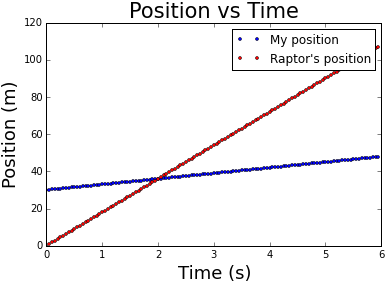
\includegraphics[width=0.40\textwidth]{positionplot.png}        
\caption{Plot of position as a function of time.}
\label{position}

\end{figure}

\begin{figure}          		
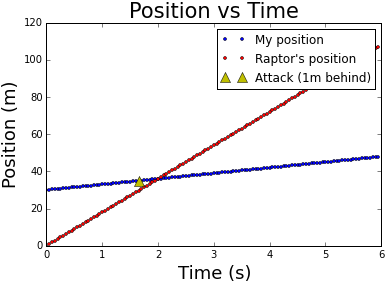
\includegraphics[width=0.40\textwidth]{attackplot.png}        
\caption{Same plot as Figure~\ref{position} with point of attack shown when raptor is 1 meter behind.}
\label{attack}

\end{figure}
%%%%%%%%%%%%%%%%%%%%%%%%%%%%%%%%%%%%%%%%%%%%%%%%%%%%%%%%%%%%%%%%%%%%%%%%%%%%%%%%
\section{Analysis}
\subsection{Problem 1}
Using the given values, and substituting into equation~\ref{positioneqn}, the resulting values for positions for the person and the raptor, X, were plotted along the y-axis as a function of time yielding Figure~\ref{position}. The plot shows the approximate time and position when the two paths cross, thereby showing when the raptor will catch up to the person. 
\subsection{Problem 2}
To find the exact time when the raptor will catch up, a for/if loop in Python was used to find when the person's position X and raptor position X2 equal one another. The program found that X=X2 at 36.00 meters at 2.0 seconds. 
\subsection{Problem 3}
The raptor will start attacking 1 meter away so at 35 meters so to find the time at this position, the same loop in Python was used with the addition of an 'and' condition to find X in the range (34.9-35.0) since there were no X exactly at 35.0. This returned a time t=1.65 seconds at 34.95 meters.
\subsection{Problem 4}
When the raptor is 1 meter away, it will attempt to bite the person. The first attempt has 20\% success, second at 15\%, and third at 7\%. The probability that it fails all three times can be calculated algebraically using equation~\ref{probability}. The result was 63.24\% chance the person will get away. The probability can also be tested in a survey of random points using a for loop and nested if statements. The first if statement tested for random points under 0.8 corresponding to the 80\% chance of survival. The second tested for points under 0.85 and third for points less than 0.93. All three tested independent random points. The total points that made it through all three tests represent the percentage of people who survived all three attack attempts. The resulting percentage gets closer to the algebraic answer as the number of test points increases. 


%%%%%%%%%%%%%%%%%%%%%%%%%%%%%%%%%%%%%%%%%%%%%%%%%%55
\section{Equations}
Kinematic equation to determine the position (x), as a function of time (t) given x\textsubscript{o}= 30 m and v\textsubscript{o}= 3 m/s:
\begin{eqnarray}
\label{positioneqn}
x&=x_o+v_ot \\
&= 30+3t 
\end{eqnarray}
Equation (2) is used to calculate x plotted on the y-axis as a function of the independent variable t plotted on the x-axis.\\
Calculation of probability given first attack is 20\% chance of success, second is 15\% and third and last attempt is 7\% chance:
\begin{eqnarray}
\label{probability}
P &= (1-0.20)(1-0.15)(1-0.07) \\
&= 0.63 \\
&= 63\%
\end{eqnarray}
%%%%%%%%%%%%%%%%%%%%%%%%%%%%%%%%%%%%%
\section{Conclusions}
	Based on the plots (Fig~\ref{position} and Fig~\ref{attack}) there is a very slim chance for the person to evade the raptor, given only 2 seconds before it catches up to the person at 36 meters. This chance is decreased with the fact that the raptor will start attacking 1 meter before that with three attempts before it gives up. However, it's still hopeful!
%%%%%%%%%%%%%%%%%%%%%%%%%%%%%%%%%%%%%%%%%%%%%%%%%%%%%%%%%%%%%%%%%%%%%%%%%%%%%%%%
\end{document}
%%%%%%%%%%%%%%%%%%%%%%%%%%%%%%%%%%%%%%%%%%%%%%%%%%%%%%%%%%%%%%%%%%%%%%%%%%%%%%%%
